\section{Sistemi Multi-Robot}

Iniziamo con i sistemi multi-robot, in particolare cominceremo con il problema di controllo di formazione. Consideriamo $N$ robot con dinamica a integratore
\begin{equation}
\dot{x}_i(t) = u_i(t), \qquad \forall i =1, \dots, N
\end{equation}
in cui abbiamo che 
\begin{itemize}
\item $x_i \in \mathbb{R}^n$ la posizione del robot $i$ (con $n=2$ o $n=3$).
\item $u_i$ la velocit\`a del robot $i$
\end{itemize}

Discretizzando l'equazione differenziale con $T_s$ tempo di campionamento si ha
\begin{equation}
x_i(t+1) = x_i(x) + T_s u_i(t)
\end{equation}

Gli obiettivi di controllo sono definiti attraverso un potenziale artificale $J(x)$ che viene minimizzato in modo da definire la legge di controllo
\begin{equation}
u_i(t) = -K_p \nabla_i J(x)
\end{equation}
in cui $K_p$ \`e un parametro detto \textit{guadagno}.

A tempo continuo si ha quindi un \textit{sistema a gradiente}
\begin{equation}
\dot{x}_i(t) = -K_p \nabla_i J(x), \qquad \forall i = 1, \dots, N
\end{equation}
che altro non \`e che la versione tempo discreto del metodo del gradiente.
A tempo discreto si ha
\begin{equation}
x_i(t+1) = x_i(t) - T_s K_p \nabla_i J(x), \qquad \forall i =1, \dots, N
\end{equation}
ovvero, praticamente, il metodo del gradiente per minimizzare $J(x)$ con passo di discesa dipendente dal tempo di campionamento e dal guadagno.

\subsection{Controllo di Formazione}

L'obiettivo \`e quello di portare i robot in una certa formazione desiderata specificata in termini di:
\begin{enumerate}
\item \textit{Posizioni assolute:} in cui l'insieme delle configurazioni desiderate \`e dato da $\mathbb{S} = \{ x: x_i = \xi_i, i = 1, \dots, N\}$ dove $\xi_i$ \`e la posizione desiderata per il robot $i$.
\item \textit{Posizioni relative:} in cui l'insieme delle configurazioni desiderate \`e dato da $\mathbb{S} = \{x : x_i - x_j = \xi_{ij}, \forall \{i,j\} \in \mathcal{E} \}$ dove $\xi_{ij}$ \`e la posizione relativa desiderata tra i robot $i$ e $j$.
\item \textit{Distanze relative:} in cui l'insieme delle configurazioni desiderate \`e dato da $\mathbb{S} = \{x: ||x_i - x_j|| = \delta_{ij}, \forall \{i,j\} \in \mathcal{E} \}$ dove $\delta_{ij}$ \`e la distanza desiderata tra i robot $i$ e $j$.
\end{enumerate}

\begin{itemize}
\item \textbf{Posizioni assolute}: Definiamo il potenziale come 
\begin{equation}
J(x) = \sum_{i=1}^N J_i(x_i(t))
\end{equation} dove 
\begin{equation}
J_i(x) = \frac{1}{2} ||x_i(t) - \xi_i ||^2
\end{equation} che ha un unico punto di minimo quando $x_i = \xi_i$. La legge di controllo \`e
\begin{equation}
u_i(t) = - K_p (x_i(t) - \xi_i) = K_p (\xi_i - x_i(t))
\end{equation} Questo va bene in un contesto \textit{centralizzato} in cui un decisore centrale dice a ciascun robot dove andare. Inoltre ogni robot deve operare nello stesso sistema di coordinate, dal momento fanno uso delle posizioni assolute.
In questo caso non serve coordinamento per raggiungere la formazione ma il coordinamento \`e necessario per altri obiettivi (mantenimento della connessione, evitamento di collisioni,...) esplicitati attraverso l'aggiunta di termini al potenziale.

\item \textbf{Posizioni relative}: In questo caso si scrive
\begin{equation}
J(x) = \sum_{\{ij\} \in \mathcal{E}} \frac{1}{2} ||x_i(t) - x_j(t) - \xi_{ij}||^2
\end{equation} che ha un unico punto di minimo quando $x_i(t) - x_j(t) = \xi_{ij}$.
La legge di controllo \`e
\begin{equation}
u_i(t) = -K_p \sum_{j \in N_i} (x_i(t) - x_j(t) - \xi_{ij}) = K_p \sum_{j \in N_i} (\xi_{ij} + x_j(t) - x_i(t))
\end{equation} dove bisogna considerare, nella derivazione di $J(x)$, tutti i contributi dei vicini del nodo $i$-esimo. Per convenzione si ha poi $\xi_{ij} = - \xi_{ji}$.
Anche in questo caso i robot devono operare in un sistema di coordinate comune. Occorre poi fare attenzione che la formazione sia ammissibile.
\defn{\textit{Formazione ammissibile:}} Una formazione si dice ammissibile se e solo se esiste una realizzazione $x_i = x_i^*$ per $i=1, \dots, N$ che soddisfa tutti i vincoli $x_i^* - x_j^* = \xi_{ij}, \forall \{i,j\} \in \mathcal{E}$.

\begin{mybox}[breakable]{green}{\exmp{\textit{Formazione ammissibile in un triangolo}}}
\label{exmp:formaz}
In un grafo di questo tipo
\begin{center}
\begin{tikzpicture}[-, >=stealth', auto, semithick, node distance=3cm]
\tikzstyle{every state}=[fill=white,draw=black,thick,text=black,scale=1]
    \node[shape=circle,draw=black] (1) at (-1,-1) {$1$};
    \node[shape=circle,draw=black] (2) at (0,0) {$2$};
    \node[shape=circle,draw=black] (3) at (1,-1) {$3$};
    \path (1) edge node {} (2);
    \path (2) edge node {} (3);
    \path (3) edge node {} (1);
\end{tikzpicture}
\end{center}
si ha
\begin{equation*}
\begin{cases}
x_1 - x_2 = \xi_{12} \\
x_2 - x_3 = \xi_{23} \\
x_3 - x_1 = \xi_{31}
\end{cases}
\end{equation*} 
sommando le tre condizioni
\begin{equation*}
(x_1 - x_2) + (x_2 - x_3) + (x_3 - x_1) = \xi_{12} + \xi_{23} + \xi_{31}
\end{equation*} da cui si ha che la formazione \`e ammissibile se e solo se
\begin{equation*}
0 = \xi_{12} + \xi_{23} + \xi_{31}
\end{equation*}
\end{mybox}
Condizioni analoghe valgono per tutti i cicli del grafo: \textit{una formazione \`e ammissibile} \textbf{se e solo} se il sistema di equazioni lineari
\begin{equation}
x_i - x_j = \xi_{ij}, \quad \forall \{i,j\} \in \mathcal{E}
\end{equation} ammette soluzione.
Questo pu\`o essere scritto in termini della matrice di incidenza $M$ del grafo:
\begin{equation}
Mx = \xi
\end{equation} dove $Mx$ \`e il vettore di tutte le differenze $x_i - x_j$ e $\xi$ \`e il vettore delle differenze desiderate $\xi_{ij}$.
In definitiva una formazione \`e ammissibile se e solo se 
\begin{equation}
\text{rank} [M | \xi] = \text{rank}(M)
\end{equation}
Se il grafo \`e connesso e la formazione \`e ammissibile allora tutte le realizzazioni $x_i = x_i^*, i=1,\dots,N$ che soddisfano i vincoli differiscono solo per una traslazione $\tau$. Infatti si ha
\begin{equation}
x_i^* - x_j^* = \xi_{ij}, \forall \{i,j\} \in \mathcal{E}
\end{equation} se si effettua una traslazione $x_i^* \to x_i^* + \tau, \forall i$ si ha
\begin{equation}
x_i^* + \tau - (x_j^* + \tau) = x_i^* - x_j^* = \xi_{ij}
\end{equation} ovvero che la formazione viene specificata a meno di una traslazione arbitraria. Questo \`e un vantaggio qualora si voglia far muovere i robot in formazione di una traslazione $\tau$ uguale per tutti.
Dovendo mantenere i vincoli si ha che una rotazione della formazione non \`e invece ammessa, e questo \`e uno dei motivi per cui analizziamo anche le distanze relative.
\end{itemize}
\begin{itemize}
\item \textbf{Distanze relative}: Anche qui il potenziale \`e definito tra coppie di nodi
\begin{equation}
J(x) = \sum_{\{i,j\} \in \mathcal{E}} J_{ij} (x_i, x_j)
\end{equation} che si pu\`o specificare ad esempio come
\begin{equation}
J_{ij} (x_i, x_j) = \frac{1}{4} \Big ( ||x_i - x_j||^2 - \delta_{ij}^2 \Big)^2
\end{equation} che per\`o \`e un oggetto non convesso. La legge di controllo quindi \`e data da
\begin{equation}
u_i(t) = -K_p \sum_{j \in N_i} \Big ( ||x_i -x_j||^2 - \delta_{ij} \Big )(x_i - x_j)
\end{equation} In questo caso non \`e necessario un sistema di coordinate globali ma ciascun robot pu\`o operare nel suo sistema di coordinate. Anche in questo caso occorre stare attenti che la formazione specificata sia ammissibile.
\begin{center}
   \begin{tikzpicture}[scale=0.7]
    \begin{axis}[
    axis lines = center,
    axis on top, scale only axis,
    xlabel = $x_i - x_j$,
    ylabel = {$J_{ij}(x_i,x_j)$},
    xmax = {3},
    xmin = {-3},
    ymax = {2},
    ymin = {0},
    restrict y to domain = 0:2,
    yticklabels={,,},
    xticklabels={,,},
    clip=false,
]
\addplot [
    domain=-3:3,
    samples=100,
    color=black,
]
{x^4 -2*x^2 + 1};
\node[below=3pt] at (-1,0) {$-\delta_{ij}$};
\node[below=3pt] at (1,0) {$\delta_{ij}$};
\end{axis}
\end{tikzpicture}
\end{center}
\begin{mybox}[breakable]{green}{}
Riprendendo l'esempio \ref{exmp:formaz} si ha che le le distanze desiderate
\[
\begin{cases}
||x_1 - x_2|| = \delta_{12} \\
||x_2 - x_3|| = \delta_{23} \\
||x_1 - x_3|| = \delta_{13}   
\end{cases}
\] inducono che la formazione sia ammissibile se e solo se valgono le disuguaglianze triangolari
\[
\begin{cases}
\delta_{12} + \delta_{23} \leq \delta_{13} \\
\delta_{12} + \delta_{13} \leq \delta_{23} \\
\delta_{13} + \delta_{23} \leq \delta_{12}
\end{cases}
\]
\end{mybox}
\end{itemize}
In generale per\`o, date le distanze $\delta_{ij}$ capire se la formazione \`e ammissibile non \`e banale come nell'esempio, dovendo risolvere un sistema di equazioni non-lineari. Normalmente si procede al contrario: prima si assegna una realizzazione $x_i = x_i^*$ e poi si calcolano le distanze (in questo modo la formazione \`e ammissibile per costruzione).
Anche se la formazione \`e ammissibile e il grafo \`e connesso la formazione risultante pu\`o essere non ben definita.

\begin{mybox}[breakable]{green}{\exmp{\textit{Definizione di formazioni}}}
Consideriamo due grafi
\begin{center}
\begin{tikzpicture}[-, >=stealth', auto, semithick, node distance=3cm]
\tikzstyle{every state}=[fill=white,draw=black,thick,text=black,scale=1]
    \node[shape=circle,draw=black] (1) at (-1,-1) {$1$};
    \node[shape=circle,draw=black] (2) at (0,0) {$2$};
    \node[shape=circle,draw=black] (3) at (1,-1) {$3$};
    \node[shape=circle,draw=black] (4) at (0,-2) {$4$};
    \path (1) edge node {} (2);
    \path (2) edge node {} (3);
    \path (3) edge node {} (4);
    \path (4) edge node {} (1);
    
    \node[shape=circle,draw=black] (5) at (4,-1) {$x$};
    \node[shape=circle,draw=black] (6) at (5,0) {$y$};
    \node[shape=circle,draw=black] (7) at (6,-1) {$z$};
    \node[shape=circle,draw=black] (8) at (5,-2) {$w$};
    \path (5) edge node {} (6);
    \path (6) edge node {} (7);
    \path (7) edge node {} (8);
    \path (8) edge node {} (6);
    \path (7) edge node {} (5);
    \path (8) edge node {} (5);
\end{tikzpicture}
\end{center}
Nel primo caso la formazione non \`e ben definita. Applicando una trasformazione non rigida (deformazione), ad esempio avvicinando i nodi $1$ e $3$ si otterrebbe un rombo. La formazione \`e quindi non rigida. Come si rende rigida? Specificando i vincoli sulle diagonali, come nel secondo grafo, in cui mantenendo le distanze si possono effettuare traslazioni e/o rotazioni.
\end{mybox}

\subsubsection{Rigidezza}
Specificare in termini di distanze relative permette quindi anche di ammettere rotazioni della formazione. 
\defn{\textit{Formazione globalmente rigida:}} Una formazione si dice \textbf{globalmente rigida} se, data una realizzazione $x_i = x_i^*, i = 1, \dots, N$ che soddisfa i vincoli
\begin{equation}
||x_i^* - x_j^*|| = \delta_{ij}
\end{equation} tutte le altre realizzazioni che soddisfano i vincoli differiscono solo per una trasformazione rigida (traslazione e/o rotazione).
Saremmo interessati a formazioni globalmente rigida ma studiare questa propriet\`a \`e complicato, soprattutto in $3$ dimensioni. Di solito si considera la condizione pi\`u debole di rigidezza locale.

\defn{\textit{Formazione localmente rigida:}} Una formazione si dice \textbf{localmente rigida} se e solo se tutte le trasformazioni infinitesime che preservano le distanze sono rigide (ovvero non ammettono deformazioni). Questa propriet\`a al contrario della rigidezza globale pu\`o essere studiata in modo semplice.
\begin{mybox}[breakable]{green}{\exmp{\textit{Rigidezza di una formazione}}}
\begin{center}
\begin{tikzpicture}[-, >=stealth', auto, semithick, node distance=3cm]
\tikzstyle{every state}=[fill=white,draw=black,thick,text=black,scale=1]
    \node[shape=circle,draw=black] (1) at (-1,-1) {$1$};
    \node[shape=circle,draw=black] (2) at (0,0) {$2$};
    \node[shape=circle,draw=black] (3) at (1,-1) {$3$};
    \node[shape=circle,draw=black] (4) at (0,-2) {$4$};
    \path (1) edge node {} (2);
    \path (2) edge node {} (3);
    \path (3) edge node {} (4);
    \path (4) edge node {} (1);
    \path (1) edge node {} (3);
\end{tikzpicture}
\end{center}
Questa formazione non \`e rigida in $\mathbb{R}^3$, dal momento che pu\`o essere piegata unendo i nodi $2$ e $4$. La rigidezza dipende quindi dallo spazio euclideo che si considera. Se si avessero dei robot volanti dovremmo tenerlo in considerazione. Inoltre questa formazione si dice \textit{localmente rigida} in $\mathbb{R}^2$ dal momento che non si possono applicare deformazioni infinitesime (deformazioni con continuit\`a) senza modificare le distanze. Se si sovrapponesse il nodo $2$ con il nodo $4$
\begin{center}
\begin{tikzpicture}[-, >=stealth', auto, semithick, node distance=3cm]
\tikzstyle{every state}=[fill=white,draw=black,thick,text=black,scale=1]
    \node[shape=circle,draw=black] (1) at (-1,-1) {$1$};
    \node[shape=circle,draw=black] (2) at (0,0) {$2$};
    \node[shape=circle,draw=black] (3) at (1,-1) {$3$};
    \path (1) edge node {} (2);
    \path (2) edge node {} (3);
    \path (1) edge node {} (3);
\end{tikzpicture}
\end{center}
si avrebbe che questa non \`e una \textit{globalmente rigida} perch\`e esistono altre realizzazioni con formazioni diverse con le stesse distanze.
\end{mybox}
Fissata una realizzazione $x_i = x_i^*$ che soddisfa i vincoli, $\forall \{i,j\} \in \mathcal{E}$
\begin{equation}
||x_i^* - x_j^*|| = \delta_{ij}
\end{equation} si considerano informazioni infinitesime
\begin{equation}
\begin{cases}
x_i = x_i^* + dx_i \\
x_j = x_j^* + dx_j
\end{cases}
\end{equation} applicando una trasformazione quadratica sui vincoli (per la differenziabilit\`a) e derivando entrambi i membri si ha
\begin{equation}
2( dx_i - dx_j)^\intercal ( x_i^* - x_j^*) = 0
\end{equation} quindi per mantenere la distanza costante tale variazione deve essere nulla. Le deformazioni infinitesime che preservano le distanze devono soddisfare i vincoli
\begin{equation}
( dx_i - dx_j)^\intercal ( x_i^* - x_j^*) = 0, \qquad \forall \{i,j\} \in \mathcal{E}
\end{equation} Questo \`e un sistema di equazioni lineari che pu\`o essere scritto come, definendo il vettore delle deformazioni complessive $dx = [dx_1, \dots, dx_N]^\intercal $ e fissando la \textbf{matrice di rigidezza} $R(x^*)$, con $x^* = [x_1^*, \dots, x_N^*]^\intercal $ si ha
\begin{equation}
R(x^*) dx = 0
\end{equation}
La formazione \`e quindi localmente rigida nella realizzazione $x_1^*, \dots, x_N^*$ se e solo se tutte le soluzioni $dx$ del sistema sono trasformazioni rigide (ovvero tutte le distanze sono preservate).\\
In $2D$ si hanno $2N$ (incognite) gradi di libert\`a mentre in $3D$ se ne hanno, ovviamente, $3N$. Dovendo ammettere solo trasformazioni rigide, ad esempio, in $2D$ devono rimanere $3$ gradi di libert\`a. Sempre in $2D$ si ha che la formazione \`e localmente rigida se e solo se il sistema ha $\infty^3$ soluzioni. Questo \`e vero se e solo se
\begin{equation}
\text{rank }R(x^*) = 2N - 3
\end{equation} dove $3$ sono i gradi di libert\`a associati a una trasformazione rigida (un angolo e due traslazioni su $x,y$).
In $3D$ si ha che la formazione \`e localmente rigida se e solo se si ha $\infty^6$ (avendo 6 gradi di libert\`a, $x,y,z$ e gli angoli di Eulero) quindi se e solo se 
\begin{equation}
\text{rank }R(x^*) = 3N - 6
\end{equation}
\textit{La rigidezza locale si studia quindi con una condizione di rango.}

\subsection{Mantenimento della connettivit\`a ed evitamento delle collisioni}

\subsubsection{Mantenimento della connettivit\`a}
In situazioni reali la presenza di un collegamento $\{i,j\} \in \mathcal{E}$ tra due robot dipende dalle loro posizioni $x_i(t)$ e $x_j(t)$. Questo pu\`o essere dovuto a varie ragioni (raggio di comunicazione limitato, visibilit\`a limitata, ...) e in pratica si ha un grafo tempo-variante $\mathcal{G} = (\mathcal{N}, \mathcal{E}(t))$. Studiamo il modello pi\`u semplice \`e dato da
\begin{equation}
\{i,j\} \in \mathcal{E}(t) \iff ||x_i(t) - x_j(t)|| \leq \rho
\end{equation} con $\rho$ raggio di comunicazione. Il nostro obiettivo \`e:
Supponendo $\mathcal{G}(0) = (\mathcal{N}, \mathcal{E}(0))$ connesso vogliamo $\mathcal{G}(t)$ connesso $\forall t$. \\
\textbf{Idea semplice}: se inizialmente \`e connesso l'idea \`e quella di continuare a preservare la connettivit\`a, considerando un sottoinsieme $\mathcal{E}_f \subseteq \mathcal{E}(0)$ di archi t.c. $\mathcal{G}_f = (\mathcal{N}, \mathcal{E}_f)$ sia connesso e si impone che
\begin{equation}
\mathcal{E}_f \subseteq \mathcal{E}(t), \qquad \forall t
\end{equation} Quindi si costruisce l'insieme dei vincoli (insieme di stati ammissibili) $\mathbb{V}_{con}$ come
\begin{equation}
\mathbb{V}_{con} = \{ x: ||x_i - x_j || \leq \rho, \quad \forall \{i,j\} \in \mathcal{E}_f \}
\end{equation} e l'obiettivo diventa $x(t) \in \mathbb{V}_{con}, \forall t$. 
Per soddisfare i vincoli costruiamo un potenziale artificiale a barriera:
\begin{equation}
J_{ij}^{con} = \begin{cases}
0, & \text{se } ||x_i - x_j|| \leq \rho_0 \\
K_{con} \Big ( \frac{1}{\rho - ||x_i - x_j||} - \frac{1}{\rho - \rho_0} \Big )^\beta, & \text{se } ||x_i - x_j|| > \rho_0
\end{cases}
\end{equation} dove $\beta \in \mathbb{N}$ (tipicamente $\beta=2,3$). Il potenziale totale sar\`a quindi dato da
\begin{equation}
J(x) = J^{for}(x) + J^{con}(x)
\end{equation} dove il primo termine \`e il potenziale artificiale attrattivo per raggiungere la formazione desiderata e il secondo il potenziale artificiale repulsivo (barriera) per mantenere la connettivit\`a.
\begin{equation}
J^{con}(x) = \sum_{\{i,j\} \in \mathcal{E}_f} J_{ij}^{con} (x_i, x_j)
\end{equation} \textbf{N.B:} Questo potenziale artificiale \`e convesso perche $\mathbb{V}_{con}$ \`e un insieme convesso.

\begin{center}
   \begin{tikzpicture}[scale=0.7]
    \begin{axis}[
    axis lines = center,
    axis on top, scale only axis,
    xlabel = $x_i - x_j$,
    ylabel = {$J_{ij}^{con}$},
    xmax = {7},
    xmin = {-7},
    ymax = {3},
    ymin = {0},
    restrict y to domain = 0:3,
    yticklabels={,,},
    xticklabels={,,},
    clip=false,
    every axis x label/.style={
    at={(ticklabel* cs:1.05)},
    anchor=west,},
]
\addplot [domain=-3:3,samples=100,color=black]{0};
\addplot [
    domain=-4.95:-3,
    samples=100,
    color=black,]{2*(1/(5+x) - 1/2)^2};
\addplot [
    domain=3:4.9,
    samples=100,
    color=black,]{2*(1/(5-x) - 1/2)^2};
]
\draw[dashed,red] ({axis cs:-5,0}|-{rel axis cs:0,0}) -- ({axis cs:-5,0}|-{rel axis cs:0,1});
\draw[dashed,red] ({axis cs:5,0}|-{rel axis cs:0,0}) -- ({axis cs:5,0}|-{rel axis cs:0,1});
\node[below=3pt] at (-3,0) {$-\rho_0$};
\node[below=3pt] at (3,0) {$\rho_0$};
\node[below=3pt] at (-5,0) {$-\rho$};
\node[below=3pt] at (5,0) {$\rho$};
\end{axis}
\end{tikzpicture}
\end{center}

\subsubsection{Evitamento delle collisioni}

La distanza tra i robot deve essere sempre maggiore o uguale ad una distanza di sicurezza $\delta$ e quindi l'obiettivo sar\`a
\begin{equation}
||x_i - x_j|| \geq \delta, \quad \forall t, \quad \forall i \neq j
\end{equation} Questo obiettivo \`e relativo tra un robot e tutti gli altri (non come nel caso precedente che era limitato ai robot connessi). Questo definisce l'insieme di ammissibilit\`a $\mathbb{V}^{col}$:
\begin{equation}
\mathbb{V}^{col} = \{x: ||x_i - x_j|| \geq \delta, \forall i \neq j \}
\end{equation} Il potenziale totale \href{https://it.wikipedia.org/wiki/Dilemma_del_porcospino}{per evitare collisioni e mantenere le connessioni} \`e definito come
\begin{equation}
J(x) = J^{for}(x) + J^{con}(x) + J^{col}(x)
\end{equation} in cui $J^{col}$ \`e un potenziale artificiale repulsivo per evitare collisioni:
\begin{equation}
J^{col}(x) = \sum_{i \neq j} J_{ij}^{col} (x_i, x_j)
\end{equation}
e $J_{ij}^{col}$ \`e il duale rispetto a quello precedente
\begin{equation}
J_{ij}^{col} = \begin{cases}
0, & \text{se } ||x_i - x_j|| \geq \delta_0 \\
K_{col} \Big ( \frac{1}{||x_i - x_j|| - \delta_0} - \frac{1}{\delta - \delta_0} \Big )^\beta, & \text{se } ||x_i - x_j|| < \delta_0
\end{cases}
\end{equation} \textbf{N.B:} Questo potenziale artificiale \`e non convesso e quindi si hanno problemi legati ai minimi locali.

\begin{center}
   \begin{tikzpicture}[scale=0.7]
    \begin{axis}[
    axis lines = center,
    axis on top, scale only axis,
    xlabel = $x_i - x_j$,
    ylabel = {$J_{ij}^{col}$},
    xmax = {6},
    xmin = {-6},
    ymax = {3},
    ymin = {0},
    restrict y to domain = 0:3,
    yticklabels={,,},
    xticklabels={,,},
    clip=false,
    every axis x label/.style={
    at={(ticklabel* cs:1.05)},
    anchor=west,},
]
\addplot [
    domain=-5:-3.1,
    samples=100,
    color=black,]{2*(1/(-x-3) - 1/2)^2};
\addplot [
    domain=3.05:5,
    samples=100,
    color=black,]{2*(1/(x-3) - 1/2)^2};
]
\draw[dashed,red] ({axis cs:-3,0}|-{rel axis cs:0,0}) -- ({axis cs:-3,0}|-{rel axis cs:0,1});
\draw[dashed,red] ({axis cs:3,0}|-{rel axis cs:0,0}) -- ({axis cs:3,0}|-{rel axis cs:0,1});
\node[below=3pt] at (-3,0) {$-\rho$};
\node[below=3pt] at (3,0) {$\rho$};
\node[below=3pt] at (-5,0) {$-\delta_0$};
\node[below=3pt] at (5,0) {$\delta_0$};
\end{axis}
\end{tikzpicture}
\end{center}

\subsubsection{Evitamento delle collisioni con ostacoli}

Anche in questo caso si definiscono potenziali artificiali repulsivi.\\
\textbf{Caso semplice}: Insieme finito di $N_o$ ostacoli $\theta_1, \dots, \theta_{N_o}$ per cui si possono calcolare in modo semplice la distanza tra un robot $i$ e il $k$-esimo ostacolo:
\begin{equation}
d(x_i, \theta_k) = \min_{x \in \theta_k} ||x_i - x||
\end{equation} Se, ad esempio, si rappresentano gli ostacoli con poligoni convessi si pu\`o definire un potenziale artificiale repulsivo per ogni ostacolo $\theta_k$ in funzione di $d(x_i, \theta_k)$ che sono della stessa forma del potenziale $J_{ij}^{col}$ (dovendo evitare di andare a collidere) che interviene quando 
\begin{equation}
d(x_i, \theta_k) \leq \hat{\delta}
\end{equation} Negli altri casi (ostacoli non convessi) si devono usare tecniche approssimate:
\begin{itemize}
\item Individuando i punti di potenziale collissioni all'interno di una circonferenza/sfera di raggio $\hat{\delta}$ (eventualmente discretizzando lo spazio di stato). Vedi Fig. \ref{fig:pedest}.
\item Definendo un potenziale artificiale repulsivo per ogni punto di collisione potenziale
\end{itemize}
\begin{figure}[htbp]
    \centering
    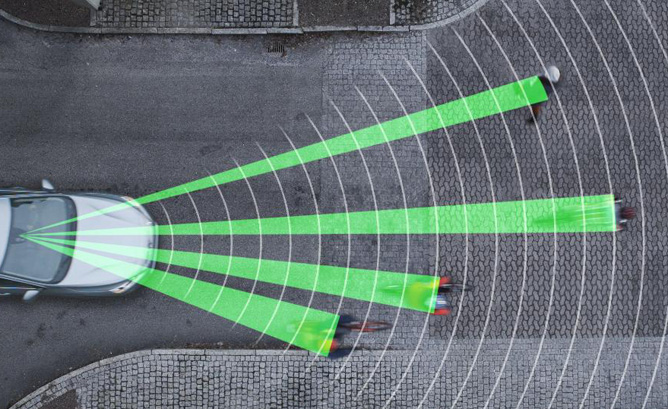
\includegraphics[scale=0.5]{img/Volvo_Pedestrian_System.jpg}
    \caption{In questo caso i punti di collisione potenziale sarebbero dati dai ciclisti.}
    \label{fig:pedest}
\end{figure}

\subsubsection{Problema dei minimi locali}
Siamo in presenza di potenziali artificiali non convessi nei casi di
\begin{itemize}
\item Controllo di formazione basato sulle distanze.
\item Evitamento delle collisioni.
\item Evitamento delle collisioni con ostacoli.
\end{itemize}
possono esserci quindi minimi locali o comunque punti stazionari tali che
\begin{equation}
\nabla_i J(x) = 0
\end{equation} ed in generale sono necessarie tecniche per risolvere il problema dei minimi locali, ad esempio:
\begin{enumerate}
\item Definire potenziali artificiali privi di minimi locali \textit{(funzioni di navigazione, potenziali armonici, programmazione dinamica,...)}. Questo va bene in casi particolare dal momento che richiede la conoscenza dell'ambiente (ostacoli + altri robot). Queste soluzioni \`e quindi adatta nei casi di ambienti statici con approccio centralizzato e pianificazione \textit{off-line}.
\item Evitare di finire nei minimi locali ad esempio fissando, mediante pianficazione di alto livello, degli obiettivi intermedi che evitano minimi locali. Anche questa tecnica \`e pi\`u adatta per pianificazione \textit{off-line}. Un'altra tecnica \`e quella di utilizzare il gradiente stocastico:
   \begin{equation}
    u_i(t) = -k_p \nabla_i J(x(t)) + \eta_i(t) 
   \end{equation} dove $\eta_i(t)$ \`e una componente stocastica introdotta in modo da permettere una certo livello di esplorazione. In questo caso si ha un compromesso tra \textit{exploitation} e \textit{exploration} (come vedremo nel reinforcement learning).
\item Usare tecniche per fuggire dai minimi locali.
\end{enumerate}

Queste due ultime tecniche richiedono un algoritmo di rivelazione, che ci dica quando si finisce in un minimo locale:
\begin{itemize}
\item \textbf{Tecniche di Wall-Following} (soprattutto in 2D per minimi locali dovuti alla presenza di ostacoli).
\item \textbf{Random Walk} (soprattutto per minimi locali non dovuti a ostacoli). La componente stocastica interviene solo quando rivelo di essere in un minimo locale. Queste tecniche portano ad algoritmi corretti in probabilit\`a (sono certo di arrivare al minimo globale, in tempo non garantito ovviamente).
\item \textbf{Ostacoli virtuali}: si introduce un ostacolo virtuale in prossimit\`a del minimo che introduce un potenziale repulsivo che fa sfuggire il robot (funziona in casi semplici).
\item \textbf{Tecniche di pianificazione ad alto livello}: algoritmi di ricerca, backtracking, subgoals...
\end{itemize}
Nella pratica si ha una combinazione di queste tecniche. Ad esempio \textit{wall following} combinato a \textit{random walk} oppure tecniche di \textit{reinforcement learning}.

\subsection{Generalizzazione ad altri modelli di robot mobili}
Abbiamo visto il modello a singolo integratore
\begin{equation}
\dot{x}_i(t) = u_i(t)
\end{equation}
ma nella pratica non \`e sempre vero che si assegni direttamente la velocit\`a (si pensi alla guida di una macchina: non si assegna la velocit\`a, si preme l'acceleratore). La difficolt\`a di questo modello \`e quindi quella di supporre che si possa assegnare $\dot{x}_i(t)$ con il controllo. Un modello pi\`u realistico \`e il modello a \textbf{doppio integratore}:
\begin{equation}
\begin{cases}
\dot{p}_i(t) = v_i(t) \\
\dot{v}_i(t) = u_i(t)
\end{cases}
\end{equation} quindi
\begin{equation}
x_i(t) = \begin{bmatrix}
p_i(t) \\
v_i(t)
\end{bmatrix}
\end{equation} con $p,v$ rispettivamente posizione e velocit\`a e $u$ accelereazione.
Si hanno quindi obiettivi di controllo:
\begin{itemize}
\item Per la posizione (es. controllo di formazione).
\item Per la velocti\`a.
\end{itemize}
Il nostro potenziale artificiale $J(x)$ sar\`a quindi costituito da diverse parti: definendo $p = [p_1, \dots, p_N]^\intercal $, $v = [v_1, \dots, v_N]^\intercal $
\begin{equation}
J(x) = K_pJ^{for}(p) + K_v J^{vel}(v) + J^{rep}
\end{equation} dove $J^{for}$ \`e il p.a. dipendente dalle posizioni per il controllo di formazione e $J^{vel}$ \`e un p.a. dipendente dalle velocit\`a per il controllo della velocit\`a. $J^{rep}$ \`e un termine che rappresenta i potenziali artificiali repulsivi aggiunti per altri obiettivi.
Tipiche scelte per $J^{vel}(v)$:
\begin{itemize}
\item Per regolare a zero la velocit\`a:
  \begin{equation}
  J^{vel}(v) = \sum_{i=1}^N ||v_i||^2
  \end{equation}
\item Per portare la velocit\`a a un valore desiderato $v^o$:
  \begin{equation}
  J^{vel}(v) = \sum_{i=1}^N ||v_i - v^o||^2
  \end{equation} ovvero allineare le velocit\`a (problema del \textit{flocking}).
\item Per allineare le velocit\`a senza specificare una velocit\`a desiderata $v^o$, ovvero un problema di consenso sulla velocit\`a:
  \begin{equation}
  J^{vel}(v) = \frac{1}{2} \sum_{\{i,j\} \in \mathcal{E}} ||v_i - v_j||^2
  \end{equation} Asintoticamente la velocit\`a di ciascun agente converge al baricentro delle velocit\`a iniziali:
  \begin{equation}
  \frac{1}{N} \sum_{i=1}^N v_i(0)
  \end{equation}
\item Per allineare la velocit\`a a quella di un leader: ad esempio il robot 1 \`e il leader e sceglie in modo indipendente il suo controllo $u_1(t)$, i robot $=2,\dots,N$ effettuano poi un consenso sulla velocit\`a.
\end{itemize}
Sia il modello singolo integratore che il doppio integratore sono modelli lineari. Nella realt\`a le dinamiche dei robot sono non linari e l'esempio pi\`u semplice \`e il \textbf{modello uniciclo}:
\begin{equation}
x_i(t) = \begin{bmatrix}
p_i(t) \\
\theta_i(t)
\end{bmatrix}
\end{equation} con $p_i \in \mathbb{R}^2$ e $\theta_i$ orientazione dell'$i$-esimo robot. Il controllo \`e dato da
\begin{equation}
u_i(t) = \begin{bmatrix}
v_i(t) \\
w_i(t)
\end{bmatrix}
\end{equation} con $v, w \in \mathbb{R}$ rispettivamente la velocit\`a di avanzamento e velocit\`a di sterzo. Nel modello dell'uniciclo si ha che, detto $p_i = [p_x^i, p_y^i]^\intercal $
\begin{equation}
\begin{cases}
\dot{p}_x^i(t) = v_i(t) \cos \theta_i(t) \\
\dot{p}_y^i(t) = v_i(t) \sin \theta_i(t) \\
\dot{\theta}_i(t) = w_i(t)
\end{cases}
\end{equation} La difficolt\`a \`e che non si pu\`o assegnare direttamente $\dot{p}_i = [\dot{p}_x^i(t), \dot{p}_y^i(t)]^\intercal $ perch\`e il vettore velocit\`a \textbf{dipende dall'orientazione}.
La strategia di controllo pu\`o essere data da questi step:
\begin{enumerate}
\item Si considera un modello semplificato a singolo integratore
    \begin{equation}
    \begin{cases}
    \dot{p}_x^i(t) = \tilde{u}_{x,i}(t) \\
    \dot{p}_y^i(t) = \tilde{u}_{y,i}(t) \\
    \end{cases} \implies \dot{p}_i(t) = \tilde{u}_i(t)
    \end{equation}
\item Si applica il metodo APF per calcolare $\tilde{u}_i(t)$.
\item Si applica un controllo di basso livello per passare dal vettore velocit\`a desiderato al controllo effettuato:
   \begin{equation}
    \tilde{u}_i(t) = \begin{bmatrix}
    \tilde{u}_{x,i}(t) \\
    \tilde{u}_{y,i}(t)
    \end{bmatrix} \to u_i(t) = \begin{bmatrix}
    v_i(t)\\
    w_i(t)
    \end{bmatrix}
   \end{equation}
\end{enumerate}
L'idea \`e: invece di controllare il punto di coordinate $(p_x^i, p_y^i)$ (che non si pu\`o controllare) si controlla un punto a distanza $b$:
\begin{equation}
\begin{cases}
\tilde{p}_x^i(t) = p_x^i(t) + b\cos \theta_i(t) \\
\tilde{p}_y^i(t) = p_y^i(t) + b\sin \theta_i(t)
\end{cases}
\end{equation} da cui
\begin{align*}
\frac{d}{dt} \tilde{p}_x^i(t) &= \frac{d}{dt} p_x^i(t) + b \cos \theta_i(t) = \dot{p}_x^i(t) - b \sin \theta_i(t) \dot{\theta}_i(t) = \\
&= v_i(t) \cos \theta_i(t) - b w_i(t) \sin \theta_i(t)
\end{align*} e infine
\begin{equation}
\begin{cases}
\frac{d}{dt} \tilde{p}_x^i(t) = v_i(t) \cos \theta_i(t) - b w_i(t) \sin \theta_i(t) \\
\frac{d}{dt} \tilde{p}_y^i(t) = v_i(t) \sin \theta_i(t) + b w_i(t) \cos \theta_i(t)
\end{cases}
\end{equation} da cui, scegliendo $u_i(t) = [v_i(t), w_i(t)]^\intercal $ si pu\`o assegnare liberamente il vettore velocit\`a:
\begin{equation}
\frac{d}{dt} \tilde{p}_i(t) = \tilde{u}_i(t)
\end{equation}
Questa tecnica prende il nome di \textbf{feedback linearization}.

\subsection{Cenni al coverage e all'esplorazione}
Supponiamo di dotare ciascun robot di un sensore con un campo di vista $FoV_i(x_i)$ dipendente dalla posizione $x_i$. L'obiettivo del problema di \textbf{coverage} \`e quello di posizionare i robot in modo che l'unione dei campi di vista
\begin{equation}
\bigcup_{i=1}^N FoV_i(x_i)
\end{equation} copra tutta l'area di interesse, supponendo di avere un numero $N$ di robot tali da coprire tutta l'area d'interesse. Se i robot hanno $FoV$ pi\`u o meno uguali allora si devono disporre i robot in modo pi\`u o meno uniforme nell'area d'interesse. Questo pu\`o essere fatto in modo distribuito sfruttando il concetto di \textbf{partizione di Voronoi}: date le posizioni $x_1, \dots, x_N$ dei robot si pu\`o associare a ogni robot $i$ una cella di Voronoi $C_i$

\begin{figure}
    \centering
    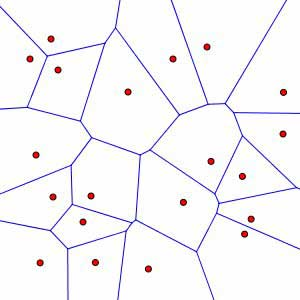
\includegraphics[scale=0.5]{img/voronoi.jpg}
    \caption{Esempio di tassellazione di Voronoi.}
    \label{fig:voronoi}
\end{figure}

in cui \begin{equation}
C_i = \{ x: ||x - x_i|| \leq ||x - x_j||, \forall j \neq i \}
\end{equation}
Le celle $C_1, \dots, C_N$ definiscono una partizione dell'area di interesse e si ha che la loro unione ci d\`a tutta l'area. Il calcolo delle partizioni di Voronoi pu\`o essere fatto in \textbf{modo completamente distribuito}, essendo necessario conoscere unicamente la propria posizione e le posizioni dei robot vicini (appartenenti a celle contigue).

\begin{algorithm}
\caption{Coverage}
\begin{algorithmic}
\REQUIRE $x_i(t), x_j(t)$
\ENSURE $j \in \mathcal{N}_i$
\FOR{$t=0,1,\dots$}
\FORALL{$\text{robot } i =1,2,\dots, N$}
\STATE $\text{Compute } C_i(t)$
\STATE $\text{Compute centroid } b_i(t)$
\STATE $\text{Apply APF method with } J(x) = \sum_{i=1}^N ||x_i - b_i||^2 + J^{other}$
\ENDFOR
\ENDFOR
\end{algorithmic}
\end{algorithm}

dove, in generale, $C_i(t)$ dipende dal tempo se i robot si muovono e il baricentro $b_i(t)$ della cella $C_i(t$ si pu\`o calcolare in forma chiusa quando l'area di interesse \`e un poligono convesso (questo implica che anche le celle siano poligoni convessi) e noi consideriamo solo questo caso.\\
Il termine $J^{other}$ rappresenta un certo numero di p.a. definiti per altri obiettivi. Si noti che $b_i(t)$ \`e una funzione di $C_i(t)$ e quindi di $x_1(t), \dots, x_N(t)$.

\begin{center}
\begin{tikzpicture}[->,node distance=1.5cm,auto,>=latex']
    \node [int] (b) {\texttt{ComputeCentroid}};
    \node (a) [above of=b] {$x_j(t)$};
    \node (d) [below of=b] {$x_i(t)$};
    \node (e) [int,right of=b,node distance=4cm] {APF};
    \node (f) [int, right of=e,node distance=3cm] {Dinamica};
    \node (g) [right of=f,node distance=2cm] {$x_i(t)$};
    \node (i) [right of=g] {};
    \draw (a) -- node {} (b);
    \draw (a) -| node {} (e);
    \draw (d) -| node {} (e);
    \draw (b) -- node {$b_i(t)$} (e);
    \draw (d) -- node {} (b);
    \draw (e) -- node {$u_i(t)$} (f);
    \draw (f) -- node {} (g);
    \draw (g) -- node {} (i);
\end{tikzpicture}
\end{center}
Questo approccio si pu\`o applicare anche a \textit{problemi di esplorazione}, in cui:
\begin{itemize}
\item Non \`e possibile coprire l'intera area di interesse con l'unione dei campi di vista.
\item L'obiettivo \`e costruire/aggiornare una mappa dell'ambiente.
\end{itemize}
L'\textbf{idea} \`e: si costruisce la partizione di Voronoi e poi ciascun robot si muove all'interno della sua cella $C_i(t)$ verso aree inesplorate ad esempio in modo da massimizzare il guadagno di informazione (definito opportunamente). \\
Servono quindi algoritmi per costruire/aggiornare in tempo reale la mappa dell'ambiente (campo di studio molto ampio, si fa con tecniche di inferenza Bayesiana). Inoltre sono necessari algoritmi per fondere in modo distribuito le mappe costruite dai singoli robot in modo da avere una mappa globale della regione esplorata (tecniche di fusione dell'informazione).

